%%\documentclass{sig-alternate}
\documentclass[letterpaper]{sig-alternate-10pt}
%%\documentclass{sig-alternate-2013}
%\newfont{\mycrnotice}{ptmr8t at 7pt}
%\newfont{\myconfname}{ptmri8t at 7pt}
%\let\crnotice\mycrnotice%
%\let\confname\myconfname%

\permission{Permission to make digital or hard copies of all or part of this work for 
personal or classroom use is granted without fee provided that copies are not made or 
distributed for profit or commercial advantage and that copies bear this notice and the 
full citation on the first page. Copyrights for components of this work owned by others 
than ACM must be honored. Abstracting with credit is permitted. To copy otherwise, or 
republish, to post on servers or to redistribute to lists, requires prior specific 
permission and/or a fee. Request permissions from permissions@acm.org.}
%%\conferenceinfo{MM'14,}{August 24--27, 2014, New York, NY, USA.}
\conferenceinfo{Conference'15,}{Date, Year, Place}
\copyrightetc{Copyright 2015 ACM \the\acmcopyr}
\crdata{Blah-blah/numbers/ ...\$15.00.\\
http://dx.doi.org/}

\clubpenalty=10000 
\widowpenalty = 10000

%\usepackage[compress]{cite}
\usepackage{cite}
%\usepackage{fixltx2e}
%\usepackage{hyperref}
%\usepackage{graphicx}
%\usepackage{varwidth}
%\usepackage{subfig}
%\usepackage{epsfig}

%%%% NORMALLY
\usepackage{subfigure}

%\usepackage{booktabs}
\usepackage{color}
%\usepackage[...]{caption}

%\usepackage{jpfigurecommands}
%% set fonts for nicer pdf view
\IfFileExists{lmodern.sty}{\usepackage{lmodern}}{}

\usepackage[T1]{fontenc}
\usepackage[latin9]{inputenc}

\usepackage{jpfigurecommands}
%\pgfplotstableread[
		format=file,
		col sep=tab,
	]{disconnect.domains-per-organization.tsv}\tableDisconnectDomainsPerOrganization

\pgfplotstableread[
		format=file,
		col sep=tab,
	]{datasets.request-status.coverage.origin.sorted.tsv}\tableDatasetsRequestStatusCoverageOriginSorted

\pgfplotstableread[
		format=file,
		col sep=tab,
	]{datasets.non-failed.classification.domain-scope.coverage.sorted.tsv}\tableDatasetsNonFailedClassificationDomainScopeCoverageSorted

\pgfplotstableread[
		format=file,
		col sep=tab,
	]{datasets.non-failed.classification.secure.coverage.sorted.tsv}\tableDatasetsNonFailedClassificationSecureCoverageSorted

\pgfplotstableread[
		format=file,
		col sep=tab,
	]{datasets.non-failed.origin-redirects.coverage.sorted.tsv}\tableDatasetsNonFailedClassificationOriginRedirectsCoverageSorted

\pgfplotstableread[
		format=file,
		col sep=tab,
	]{datasets.non-failed.disconnect.categories.coverage.external.sorted.tsv}\tableDatasetsNonFailedDisconnectCategoriesCoverageExternalSorted

\pgfplotstableread[
		format=file,
		col sep=tab,
	]{datasets.non-failed.disconnect.organizations.coverage.external.sorted.tsv}\tableDatasetsNonFailedDisconnectOrganizationsCoverageExternalSorted

\pgfplotstabletranspose[
	colnames from=Dataset
	]\tableTransposedDatasetsNonFailedRatioBucketsIsDisconnectMatchNormalizedCumulativeSorted{datasets.non-failed.ratio-buckets.is-disconnect-match.normalized.cumulative.sorted.tsv}

\pgfplotstabletranspose[
	colnames from=Dataset
	]\tableTransposedDatasetsNonFailedRatioBucketsDisconnectOrganizationsNormalizedCumulativeSorted{datasets.non-failed.ratio-buckets.disconnect-organizations.normalized.cumulative.sorted.tsv}

\pgfplotstableread[
		format=file,
		col sep=tab,
	]{datasets.non-failed.domains.ratios.sorted.tsv}\tableDatasetsNonFailedDomainsRatiosSorted

% Summaries
% TODO: see if it's possible to filter rows from tables loaded above
\pgfplotstableread[
		format=file,
		col sep=tab,
	]{datasets.request-status.coverage.origin.sorted.summary.tsv}\tableDatasetsRequestStatusCoverageOriginSortedSummary

\pgfplotstableread[
		format=file,
		col sep=tab,
	]{datasets.non-failed.classification.domain-scope.coverage.sorted.summary.tsv}\tableDatasetsNonFailedClassificationDomainScopeCoverageSortedSummary

\pgfplotstableread[
		format=file,
		col sep=tab,
	]{datasets.non-failed.origin-redirects.coverage.sorted.summary.tsv}\tableDatasetsNonFailedClassificationOriginRedirectsCoverageSortedSummary

\pgfplotstableread[
		format=file,
		col sep=tab,
	]{datasets.non-failed.classification.secure.coverage.sorted.summary.tsv}\tableDatasetsNonFailedClassificationSecureCoverageSortedSummary

\pgfplotstableread[
		format=file,
		col sep=tab,
	]{datasets.non-failed.disconnect.organizations.coverage.external.sorted.summary.tsv}\tableDatasetsNonFailedDisconnectOrganizationsCoverageExternalSortedSummary

\pgfplotstableread[
		format=file,
		col sep=tab,
	]{datasets.non-failed.disconnect.categories.coverage.external.sorted.summary.tsv}\tableDatasetsNonFailedDisconnectCategoriesCoverageExternalSortedSummary


%%% Sweden https-www

\pgfplotstableread[
		format=file,
		col sep=tab,
	]{datasets.non-failed.classification.domain-scope.coverage.sorted.sweden-https-www.tsv}\tableDatasetsNonFailedClassificationDomainScopeCoverageSortedSwedenHttpsWww

\pgfplotstableread[
		format=file,
		col sep=tab,
	]{datasets.non-failed.disconnect.organizations.coverage.external.sorted.sweden-https-www.tsv}\tableDatasetsNonFailedDisconnectOrganizationsCoverageExternalSortedSwedenHttpsWww

\pgfplotstableread[
		format=file,
		col sep=tab,
	]{datasets.non-failed.disconnect.categories.coverage.external.sorted.sweden-https-www.tsv}\tableDatasetsNonFailedDisconnectCategoriesCoverageExternalSortedSwedenHttpsWww

\pgfplotstableread[
		format=file,
		col sep=tab,
	]{datasets.request-status.coverage.origin.sorted.sweden-https-www.tsv}\tableDatasetsRequestStatusCoverageOriginSortedSwedenHttpsWww

\pgfplotstableread[
		format=file,
		col sep=tab,
	]{datasets.non-failed.origin-redirects.coverage.sorted.sweden-https-www.tsv}\tableDatasetsNonFailedClassificationOriginRedirectsCoverageSortedSwedenHttpsWww

%%% Global https-www

\pgfplotstableread[
		format=file,
		col sep=tab,
	]{datasets.non-failed.classification.domain-scope.coverage.sorted.global-https-www.tsv}\tableDatasetsNonFailedClassificationDomainScopeCoverageSortedGlobalHttpsWww

\pgfplotstableread[
		format=file,
		col sep=tab,
	]{datasets.non-failed.disconnect.organizations.coverage.external.sorted.global-https-www.tsv}\tableDatasetsNonFailedDisconnectOrganizationsCoverageExternalSortedGlobalHttpsWww

\pgfplotstableread[
		format=file,
		col sep=tab,
	]{datasets.non-failed.disconnect.categories.coverage.external.sorted.global-https-www.tsv}\tableDatasetsNonFailedDisconnectCategoriesCoverageExternalSortedGlobalHttpsWww

\pgfplotstableread[
		format=file,
		col sep=tab,
	]{datasets.request-status.coverage.origin.sorted.global-https-www.tsv}\tableDatasetsRequestStatusCoverageOriginSortedGlobalHttpsWww

\pgfplotstableread[
		format=file,
		col sep=tab,
	]{datasets.non-failed.origin-redirects.coverage.sorted.global-https-www.tsv}\tableDatasetsNonFailedClassificationOriginRedirectsCoverageSortedGlobalHttpsWww

%%% Sweden http-www

\pgfplotstableread[
		format=file,
		col sep=tab,
	]{datasets.non-failed.classification.domain-scope.coverage.sorted.sweden-http-www.tsv}\tableDatasetsNonFailedClassificationDomainScopeCoverageSortedSwedenHttpWww

\pgfplotstableread[
		format=file,
		col sep=tab,
	]{datasets.non-failed.disconnect.organizations.coverage.external.sorted.sweden-http-www.tsv}\tableDatasetsNonFailedDisconnectOrganizationsCoverageExternalSortedSwedenHttpWww

\pgfplotstableread[
		format=file,
		col sep=tab,
	]{datasets.non-failed.disconnect.categories.coverage.external.sorted.sweden-http-www.tsv}\tableDatasetsNonFailedDisconnectCategoriesCoverageExternalSortedSwedenHttpWww

\pgfplotstableread[
		format=file,
		col sep=tab,
	]{datasets.request-status.coverage.origin.sorted.sweden-http-www.tsv}\tableDatasetsRequestStatusCoverageOriginSortedSwedenHttpWww

\pgfplotstableread[
		format=file,
		col sep=tab,
	]{datasets.non-failed.origin-redirects.coverage.sorted.sweden-http-www.tsv}\tableDatasetsNonFailedClassificationOriginRedirectsCoverageSortedSwedenHttpWww

%%% Global http-www

\pgfplotstableread[
		format=file,
		col sep=tab,
	]{datasets.non-failed.classification.domain-scope.coverage.sorted.global-http-www.tsv}\tableDatasetsNonFailedClassificationDomainScopeCoverageSortedGlobalHttpWww

\pgfplotstableread[
		format=file,
		col sep=tab,
	]{datasets.non-failed.disconnect.organizations.coverage.external.sorted.global-http-www.tsv}\tableDatasetsNonFailedDisconnectOrganizationsCoverageExternalSortedGlobalHttpWww

\pgfplotstableread[
		format=file,
		col sep=tab,
	]{datasets.non-failed.disconnect.categories.coverage.external.sorted.global-http-www.tsv}\tableDatasetsNonFailedDisconnectCategoriesCoverageExternalSortedGlobalHttpWww

\pgfplotstableread[
		format=file,
		col sep=tab,
	]{datasets.request-status.coverage.origin.sorted.global-http-www.tsv}\tableDatasetsRequestStatusCoverageOriginSortedGlobalHttpWww

\pgfplotstableread[
		format=file,
		col sep=tab,
	]{datasets.non-failed.origin-redirects.coverage.sorted.global-http-www.tsv}\tableDatasetsNonFailedClassificationOriginRedirectsCoverageSortedGlobalHttpWww



%%%%%%%%%%%%%%%%%%%%%
%%NEW
\usepackage{url}

\setlength{\pdfpagewidth}{8.5in}
\setlength{\pdfpageheight}{11in}

%\newcommand{\textcolorRED}[2]{\textcolor{red}{#2}}
\newcommand{\textcolorRED}[2]{#2}

%\newcommand{\multi}[2]{\textcolor{green}{#1}}
%\newcommand{\multi}[2]{\textcolor{green}{#2}}
%\newcommand{\multi}[2]{#2}



%\DeclareCaptionType{copyrightbox}
\begin{document}


\title{Analysis of HTTPS Adoption and Third-party Tracking: \\A Swedish Perspective}
%%\title{A Swedish Perspective of HTTPS Adoption and Third-party Tracking}

%\numberofauthors{2}
%\author{
%Joel Purra\\
%Link{\"{o}}ping University, Sweden\\
%\email{mig@joelpurra.se}\\
%\and
%Niklas Carlsson\\
%Link{\"{o}}ping University, Sweden\\
%\email{niklas.carlsson@liu.se}\\
%}

\numberofauthors{2} %  in this sample file, there are a *total*
\author{
\alignauthor Joel Purra\\
       \affaddr{Link{\"o}ping University, Sweden}\\
%%       \affaddr{Link{\"o}ping, Sweden}\\
       \email{mig@joelpurra.se}
\and
\alignauthor Niklas Carlsson\\
       \affaddr{Link{\"o}ping University, Sweden}\\
%%       \affaddr{Link{\"o}ping, Sweden}\\
       \email{niklas.carlsson@liu.se}
}

\maketitle
\begin{abstract}

%Both active third-party tracking (e.g., using scripts and plugins
%embedded within visited websites) and passive tracking
%%(e.g., through network monitoring)
Today, extensive use of third-party tracking services and passive 
%%tracking through 
traffic monitoring are both used to 
%%are extensively used to 
gather knowledge about users' internet activities and interests.  
With HTTPS providing some protection against passive monitoring,
privacy concerned users are increasingly selecting services 
%that are 
provided over HTTPS.
This paper presents a measurement-driven 
analysis of the current HTTPS adoption and its relationship
to third-party tracking usage.
%%addressing the lack of careful characterizing of .
%%While HTTPS can be used to protect against some privacy concerns raised by passive monitoring, 
%prior work have not carefully characterized the HTTPS adoption 
%and third-party tracking when using HTTP and HTTPS, respectively.  This paper presents a 
%measurement analysis of the current HTTPS adoption and third-party tracking usage.  
First, we develop and release the 
software of a novel measurement framework for automated, repeatable retrieval, and analysis of websites.  
Second, we characterize the HTTPS adoption, HTTPS redirection dynamics, 
and use of secure/non-secure third-party resources from both a national (Swedish) and global perspective.  
%Across domain classes, both nationally and internationally,
%we observe low HTTPS adoption, 
%many domains that redirect to insecure resources,
%and many domains that use a mix of secure and insecure connections.
%%In total, we analyze more than 150,000 websites.  
Third, we compare and contrast the third-party tracking usage,
including the tracker service and the companies that may get access to user information,
when using HTTP and HTTPS, respectively.
%%and characterization the tracker service and the companies that may get access to user information.
%% when using HTTP and HTTPS.  
Across both national and international domain categories
we observe low-to-modest (below 50\%) HTTPS adoption,
%We also observed 
many domains that redirect to insecure domains,
%that 
or
%%and many domains 
that use a mix of secure and insecure connections 
to download the resources making up the presented website.
%or that do both.
%While Google has by far the greatest third-party coverage (more than 90\% for most website categories), 
%we have found that there are many other third-party domains that that may fly under the radar.
%domains serving third-party content that may fly under the radar.
%%Overall, we have found that users may be given a false sense of privacy when using HTTPS.  
%%They are often directed to non-secure subdomains, and even when served using HTTPS, 
The use of third-party resources is high among all considered domain categories, 
regardless if HTTPS is used or not,
suggesting that users may be given a false sense of privacy when using HTTPS.
%%In fact, both HTTPS and third-party usage is most prevalent among the most popular website, visited most often.  
%%While Google has by far the greatest third-party coverage (more than 90\% for most website categories), we have found that 
%%there are many other domains serving third-party content that may fly under the radar.
While Google has by far the greatest third-party coverage (more than 90\% for most website categories),
we have found that there are many other third-party domains that that may fly under the radar.


%Both active third-party tracking (e.g., using scripts and plugins embedded within visited websites) and passive 
%tracking (e.g., through network monitoring) are extensively used to collect information and knowledge about users 
%internet activities and interests.  While HTTPS can be used to protect against privacy concerns raised by passive 
%monitoring, prior work have not carefully studied the adoption of HTTPS and how much privacy protection against 
%third-party tracking can be gained from using HTTPS.  This paper presents a measurement analysis of the current 
%HTTPS adoption and third-party tracking usage.  First, we develop and release the software of a novel measurement 
%framework for automated, repeatable retrieval, and analysis of websites and their third-party usage and HTTPS 
%dynamics.  Second, we characterize the HTTPS adoption and use of secure/non-secure third-party resources from 
%both a national (Swedish) and global perspective.  In total, we repeatedly analyze more than 150,000 websites.  
%Third, we characterize the third-party tracking usage and the companies that may get access to user information 
%when using HTTP and HTTPS.  Overall, we have found that users may be given a false sense of privacy when using 
%HTTPS.  They are often directed to non-secure subdomains, and even when served using HTTPS, the use of third-party 
%(external) resources is high among all classes of domains, regardless if HTTP or HTTPS is used.  This is magnified 
%by third-party usage being most prevalent among the most popular website, which people visit most often.  While 
%Google has by far the greatest third-party coverage (more than 90\% for most website categories) among known 
%tracker companies, we have found that there are many other domains that also server third-party content which 
%may fly under the radar.

\end{abstract}

%% A category with the (minimum) three required fields
%%\category{C.4}{Information Systems Organization}{Performance of Systems}
%%\category{H.4}{Information Systems Applications}{Miscellaneous}
%%A category including the fourth, optional field follows...
%%\category{D.2.8}{Software Engineering}{Metrics}[complexity measures, performance measures]
%\category{C.2.2}{Information Systems Organization}{Network Protocols}[Applications] 
%%\category{H.5.1}{Multimedia Information Systems}{Video}


%%\terms{Theory}

%\keywords{Blah blah}
%%\keywords{Nonlinear streaming; Multipath streaming; HAS}

\section{Introduction}

We are living in an information society in which organizations constantly track our movements 
on the web, and use the collected (and stored) information to analyze and gain 
knowledge about us and our interests.  Website owners may use such knowledge to present personalized 
content that may better match user interests, advertisement firms may use the knowledge to sell 
targeted ads based on user interests~\cite{GEC+13,SLB+14,YZL+13,LSW+13}, media analytics firms may use the data to verify 
advertisement-related statistics, and data brokers may package and sell the user data 
inferred from the user interests~\cite{Armo14}.

Web usage is both actively and passively tracked.  With active tracking, 
third-party scripts and plugins embedded within the visited websites
%%for example,
are typically used to extract and collect information about a user's every click, 
the time spent on each page (even if inactive), and information
that can be used to uniquely identify each browser and client
(including operating system, window size, screen resolution, installed fonts, etc.).
%%the user environment (including operating system, window size, 
%%screen resolution, and color depth), mouse movements, scrollbar location, installed fonts, 
%%plugins, extensions, and any potential error reports, for example.  
While some trackers allow advanced fingerprinting through collection of client-side information,
much tracking is achieved through server-side tracking of the download of
relatively simple third-party contents such as CSS files, customized fonts, 
or javascript libraries that does not include tracking code themselves~\cite{AEE+14,MPS+13,MaMi12,RoKW12,NIK+12}.  
%All external resources are considered trackers, even if code isn't executed on the client. 
%CSS and fonts for example are major trackers for Google, as well as their hosting of javascript 
%libraries (such as jquery) which doesn't actually contain tracking code -- it's all passive, 
%server-side tracking and often served over HTTPS.
User activities can also be 
%passively 
tracked through 
passive traffic monitoring within the network or at a cloud-operated data center hosting some of the content.
%%can also be performed by passive monitoring of the end-to-end network traffic. 
%%network traffic can be monitored at any point in the network or at a cloud-operated data center, for example,
Here, unencrypted HTTP data such as header information 
%(e.g., URLs, previously visited websites, and the client's browser, OS, and cookies)
as well as application specific information (including information sent to third-party trackers)
could be used to identify users and track their web sessions.
%%allowing user actions and user interests to be inferred from the traffic patterns, HTTP-related information (such as URLs of 
%%visited websites, previously visited websites, the client's browser, operating system, and cookies, for example), 
%%and any other application specific information (including information sent to third-party trackers).

In parallel with a trend towards increased user tracking, 
there has also been an increase in the number of services that use HTTPS.  
HTTPS helps secure the end-to-end communication between the client and server
%%help 
and limits the information that can be passively collected along the network path. 
However, it does not protect against tracking enabled through embedded 
third-party content or tracking codes.  
When considering the current state-of-the art, and these trends in particular, 
a number of important question arise:  What is the status of the current HTTPS adoption?  
How much third-party tracking is deployed?  Does third-party tracking usage differ for 
%%early 
domains adopting HTTPS?  And, perhaps most importantly, how much privacy and protection against 
third-party tracking can be gained from conscious use of HTTPS?  
As of today, there have only been some preliminary works touching upon the first 
two of these questions~\cite{BuMS11,NFL+14}, 
but no work has carefully addressed all four questions.

To help address these important and un-answered questions, this paper presents 
a novel measurement methodology and analysis of the current HTTPS and third-party tracking usage.  
Leveraging Swedish domain knowledge, the study presents results from both a national (Swedish) 
and global perspective.
%% (using globally popular service, for example).  
The paper makes three main contributions.

First, we develop and release the software of a 
%novel
measurement framework for automated, 
repeatable retrieval, and analysis of websites and their third-party usage and 
HTTPS dynamics.\footnote{Both the open source project and datasets used in the paper 
are made public with this paper,
and can be found here:
%Code and datasets can be found here: 
\url{http://joelpurra.com/projects/masters-thesis/}.}  
The software is built on open source software, uses a non-modified ``standard'' headless browser, 
and stores results into standardized HAR format.  To capture HTTPS adoption and redirections, 
domains are visited using both \texttt{http} and \texttt{https}, with and without the \texttt{www} prefix. 
Third-party resource usage is captured through post processing (including comparison with the tracker 
lists of the popular privacy tool \texttt{disconnect.me}\footnote{Disconnect, \url{https://disconnect.me/}, May 2015.}) 
and public suffix lists are used to identify domains and subdomains.

Second, we characterize the HTTPS adoption and use of secure/non-secure third-party resources from 
both a Swedish and global perspective.  
%%We find that the HTTPS adoption among globally popular 
%%websites (10-30\%) and lists of both popular and important Swedish 
%%websites (15-50\%) is much higher than for random domains (less than 1\%). 
Although it appears that the globally most popular websites (10-30\% HTTPS adoption)
and popular and important Swedish websites (15-50\%) are much further along in their adoption
than random domains (less than 1\% adoption), the low overall values suggest 
that most websites are susceptible to passive eavesdropping anywhere along the network path.  
To make things worse for the privacy conscious user, we have found that many websites redirect 
their users from their secure (\texttt{https}) domain to their insecure (\texttt{http}) domain, 
and many of the domains that allow use of HTTPS still 
%% secure \texttt{https} domains 
relies heavily on some (internal and third-party)
resources used for the website to be delivered insecurely.
% over HTTP,rather than over HTTPS.
%%both internal and external (third-party) 
%resources delivered over HTTP (rather than HTTPS).  
%The use of third-party resources over HTTP shows that a secure, 
%encrypted connection to a website often does not ensure privacy neither 
%against active and passive tracking.  
This is concerning as users falsely might be lead to 
believe that such “secure connection” 
%(by many browsers labeled using a padlock) 
provides protection against external tracking,
while the client may still be tracked both through third-party resource usage
and by monitoring non-secure connections. 
%still allow both active-third party tracking
%and communication over non-secure connections.
%%both passive monitoring of non-secure connections and active-third party tracking.

Third, we characterize the third-party tracking usage and the companies that may get access 
to user information when trying to download the front page of each domain 
using HTTP and HTTPS.  Overall, the use of third-party (external) 
resources is high among all domain categories, regardless if HTTP or HTTPS is used.  
For example, less than 7\% of the globally most popular domains use only internal resources.  
These numbers are even lower for the most popular Swedish websites within most websites categories, 
%but greater among random domains (10-30\%), 
suggesting that users' activities often can be tracked 
through third-party resource usage.  In fact, most websites also have at least one {\em known} 
tracker present: 53-72\% of random domains, 88-98\% of top websites, and 78-100\% of websites 
in the different Swedish top-categories.  While Google has by far the greatest third-party 
coverage among known tracker companies (e.g., Google has trackers on more than 90\% of the 
websites within the majority of the website categories considered here), we have found that 
there are many other third-party domains that may fly under the radar.  
For example, Disconnect's blocking list only detects 10\% of the 
%external 
third-party primary domains.  
With most of these non-blocked third-party entries being third-party content providers, which are 
known to keep track of users across services, we expect that there will be a continued 
battle for the knowledge about our web activities.

The remainder of the paper is organized as follows. 
%Section~\ref{sec:background} gives a brief background on online tracking.  
Our methodology and measurement framework are 
described in Section~\ref{sec:method}.  Section~\ref{sec:https} presents our 
characterization results for HTTPS adoption and client redirections between 
secure and non-secure resources.  Section~\ref{sec:tracking} characterizes the 
third-party tracking landscape and how it differs between secure and non-secure 
domains. Finally, Section~\ref{sec:related} discusses related works, before 
Section~\ref{sec:conclusions} concludes the paper.

%%%%%%%%%%%%%%%%%%%%%%%%%%%%%%%%%%%%%%%%%%%%%%%%%%%%%%%%%%%%
%%%%%%%%%%%%%%%%%%%%%%%%%%%%%%%%%%%%%%%%%%%%%%%%%%%%%%%%%%%
%\section{Background}\label{sec:background}



%%%%%%%%%%%%%%%%%%%%%%%%%%%%%%%%%%%%%%%%%%%%%%%%%%%%%%%%%%%%
%%%%%%%%%%%%%%%%%%%%%%%%%%%%%%%%%%%%%%%%%%%%%%%%%%%%%%%%%%%

%\begin{table*}[t]
%\centering
%\caption{Summary of domain lists.}
%\label{tab:domains}
%{\small
%\begin{tabular}{|l|c|r|l|r|r|}\hline
%\hline %% closing line
%Domain list       & Date       & Total size  & Selection & Selection size & Unique\\\hline
%.SE health status & 2014-03-27 & 980         & curated   & 915            & 915   \\\hline
%.se zone          & 2014-07-10 & 1,318,000   & random    & 100,000        & 100,000 \\\hline
%.dk zone          & 2014-07-23 & 1,260,000   & random    & 10,000         & 10,000 \\\hline
%.com zone         & 2014-08-27 & 114,178,000 & random    & 10,000         & 10,000 \\\hline
%.net zone         & 2014-08-27 & 15,096,000  & random    & 10,000         & 10,000 \\\hline
%reach50           & 2014-09-01 & 50          & top       & 50             & 50 \\\hline
%Alexa Top 1M      & 2014-09-01 & 1,000,000   & top       & 10,000         & 9,986 \\\hline
%                  &            &             & random    & 10,000         & 9,959 \\\hline
%                  &            &             & all .se   & 3,364          & 3 364 \\\hline
%                  &            &             & all .dk   & 2,637          & 2,637 \\\hline
%Total             &            & 132,852,050 &           & 156,907        & 156,045 \\\hline
%\end{tabular}}
%\vspace{-0pt}
%\end{table*}

\section{Methodology}\label{sec:method}

Our measurement campaign is as follows: 
we visit the front page of each domain, 
using both \texttt{http} and \texttt{https},
from a large set of domains.  
For each case we consider both the domain with and without the \texttt{www} prefix.  
Using the tool developed in this project, 
the front page of each domain is downloaded and parsed using the headless \texttt{phantomjs} browser 
the same way the users' browser would.
%\footnote{
%%Since the headless browser does not have a display window,
%As part of the validation process,
%the tool creates an image of the full website after the download is complete,
%but does not display the results to any user.}  
The URL of each requested resource is extracted, 
and then associated with the domain it was loaded from.  
Finally, each object and domain is classified and prepared 
for post processing and analysis.

%In this work, 
%We perform a large-scale measurement campaign in which 
%the front page of a large set of domains are visited
%using both \texttt{http} and \texttt{https}.
%For each cases,
%we also considered both domain variations 
%with and without the \texttt{www} prefix.
%With the tool developed in this project,
%%\footnote{The browser does not have a visible window, as it is built for automation.}
%%browser \texttt{phantomjs} downloads
%the front page of each domain is downloaded and parsed 
%using the headless 
%(without display window) 
%\texttt{phantomjs} browser 
%the same way a user's browser would.\footnote{
%Since the headless browser does not have a display window,
%As part of the validation process,
%the tool creates an image of the full website after the download is complete,
%but does not display the results to any user.}
%The URL of each requested resource is extracted, and associated with
%the domain it was loaded from. Each object and domain is classified 
%and prepared for post processing and analysis.

{\bf Swedish perspective:}  
First, our measurements are performed from computers located in Sweden.
Second, we leverage the domain lists from the .SE Health Status report\cite{LoWa12},
identified by the Internet Infrastructure Foundation (.SE) as the most important domains
to Swedish internet usage and operation.
Combined, these lists include approximately 1,000 domains in the
categories: counties (21), domain registrars (146), financial services (79), 
government-owned corporations (GOCS) (60), higher education (49), 
ISPs (20), media (33), municipalities (290), and public authorities (282).
Third, we consider the 50 global websites most visited by Swedish Internet users (reach50),
all .se domains (3,364) among the top-million globally most popular domains
according to Alexa\footnote{ Alexa (official website), \url{www.alexa.com}.}),
as well as 100K randomly selected websites within the .se domain zone.

{\bf Global baseline:}  
%To put findings in perspective and to broaden our
%conclusions we 
To put our findings into perspective and 
%as a result 
broaden our conclusions we
also consider the globally most popular websites (according to Alexa),
all .dk (Denmark) domains (2,637) among the top-million globally most popular domains,
%\footnote{Alexa (official website), \url{www.alexa.com}.}) 
and randomly selected websites from the .com, .net, and .dk (Denmark) domain zones.
Table~\ref{tab:domains} summarizes the domain lists used.
% and selection.
%%and any bias due to geographic personalization by content providers and
%%Content Delivery Networks (CDNs), for example.
%%Client in Sweden and section of websites ...

{\bf Data collection and parallelization:}
HTTP/HTTPS traffic metadata such
as requested URLs and their HTTP request/response headers have been recorded in the HTTP
Archive (HAR) data format.
During our data collection,
multiple domains have been retrieved in parallel, 
with parallelism adjusted to fit the available computer capacity. 
To reduce the risk of intermittent errors,
%% – either in software, on the network or in the remote system – 
each failed access has been retried up to two times.

\begin{table}[t]
\centering
\caption{Summary of domain lists.}
\label{tab:domains}
{\small
\begin{tabular}{|l|c|r|l|r|r|}
%%\cline{4-6}
\hline
\multicolumn{3}{|c}{Domain lists} & \multicolumn{3}{|c|}{Selection} \\\hline
List(s)           & Date       & Total size  & Type      & Size & Unique\\\hline
.SE health        & 27/3/14    & 980         & curated   & 915            & 915   \\\hline
.se zone          & 10/7/14    & 1,318,000   & random    & 100,000        & 100,000 \\\hline
.dk zone          & 23/7/14    & 1,260,000   & random    & 10,000         & 10,000 \\\hline
.com zone         & 27/8/14    & 114,178,000 & random    & 10,000         & 10,000 \\\hline
.net zone         & 27/8/14    & 15,096,000  & random    & 10,000         & 10,000 \\\hline
reach50           & 1/9/14     & 50          & top       & 50             & 50 \\\hline
Alexa 1M          & 1/9/14     & 1,000,000   & top       & 10,000         & 9,986 \\\hline
                  &            &             & random    & 10,000         & 9,959 \\\hline
                  &            &             & all .se   & 3,364          & 3 364 \\\hline
                  &            &             & all .dk   & 2,637          & 2,637 \\\hline
Total             &            & 132,852,050 &           & 156,907        & 156,045 \\\hline
\end{tabular}}
\vspace{-16pt}
\end{table}

%%{\bf Website selection:}  Different categories and different popularities ... Also Danish websites for sanity check.

{\bf Data extraction:}
A custom-built tool based on the command line JSON processor \texttt{jq}
is used to convert the HAR data into JSON-based HAR data with information about both requests and responses.
The extracted data includes protocol and hosts (e.g., from URLs), 
HTTP status, mime-type, referer and redirect values – both
for the origin domain's front page and any resources requests by it. 

{\bf Domain identification and classification:}
Each requested resource is classified across multiple dimensions, for example: 
it's mime type, if it was retrieved securely or not, and if it was downloaded 
from an internal sub-domain or from a known third-part tracker. 
%We classify each requested resource along many dimensions, 
%including its mime type, if it is retrieved securely,
%and if it is downloaded from an internal subdomain or from an known third-party tracker, for example. 
To determine the primary domain and subdomain(s) we use the 
public suffix list\footnote{Public suffix list, \url{https://publicsuffix.org/}, May 2015.} 
%(used by browser vendors to implement domain-dependent security measures)
and match domains against it.  This is important to capture the relationships
between second-level domains not open for commercial registration (e.g., \texttt{.com.br} under \texttt{.br}).  
We refer to resources requested from the main page
that are retrieved from the same domain, a subdomain
or a superdomain as {\em internal} requests.
Any other request is deemed as an {\em external} request.

{\bf Tracker identification:}
%When analyzing third-party tracking,
%it is important to note that 
Public lists of known trackers typically are incomplete and out-of-date~\cite{MPS+13, KrWi06}.
Potentially any external resource can be used for third-party tracking.
For example, 
Even static (non-script, non-executable) resources with no capabilities to
dynamically survey the users' browser or OS can track users across domains using
the referer HTTP header and customized URI's.

\begin{figure}[t]
\centering
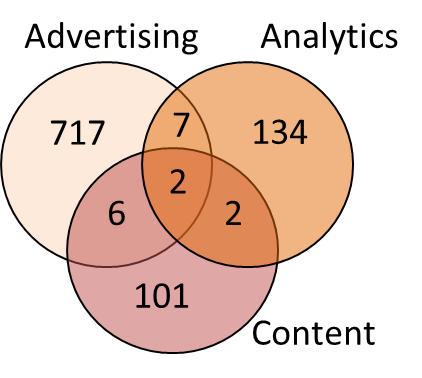
\includegraphics[width=0.23\textwidth]{venn-v00.pdf}
\vspace{-18pt}
\caption{Organizations using
different combinations of known trackers.}
\label{fig:venn}
\vspace{-16pt}
\end{figure}

With our retrieval method
%In this paper 
we do not block requests.
Instead 
%during post processing,
each resource is classified as either internal or external, 
and each URL is matched against known trackers during post processing.
%%each resource is classified either as internal or external,
%%and each URL is also matched against known trackers.
The external third-party usage provides an upper bound and
the known trackers provides a characterization of the
usage of confirmed, recognized third-party trackers.
For the tracker analysis, we use the tracker list
used by the privacy tool Disconnect.me.  This list contains 2,149 domains,
each belonging to one of 980 organizations and five tracker categories.
Figure~\ref{fig:venn} shows
%provides a Venn diagram of 
the number 
of organizations that use the three most common tracker categories: 
Advertising, Analytics, and Content.
There are also 14 organizations (with 43 total domains) 
in the social category and 3 organizations (Google, Facebook, and Twitter)
in the special ``Disconnect'' category.



%While there are public lists of known trackers, 
%%used by browser privacy tools, they 
%these lists are often incomplete and out-of-date~\cite{MPS+13, KrWi06}.
%In fact,  any external resource can be used for third-party tracking.
%For example, even for static (non-script, non-executable) resources with no capabilities to
%dynamically survey the user’s browser or OS can track users across domains using
%the referer  HTTP header and custimized URI's, for example.
%These lists are therefor perhaps best seen as lists of confirmed, recognized third-party trackers.

%In our experiments, we do not block requests.  Instead, URL are matched against known 
%trackers during post processing.  For this analysis, we use the tracker list
%used by the privacy tool Disconnect.me.  This list contains 2,149 domains,
%each belonging to one of 980 organizations and five tracker categories.
%
%ADD: STATS (maybe figure) about skew AND venn diagram of categories.

%Not all domains in the list are treated the same by Disconnect.me; 
%despite being listed as
%known trackers, the content category (A.3.6) is not blocked by default in order to not disturb
%the normal user experience too much. Most organizations are only associated with one domain,
%but some organizations have more than one domain (A.3.3). Figure 3.1 shows the number of
%organizations (out of the 980 organizations) that have a certain number of tracker domains (x
%axis). We see that 47\% (459 of 980) have at least two domains listed by Disconnect.me. Google
%(rightmost point) alone has 271 domains and Yahoo has 71. Some organizations have their
%domains categorized in more than one category, as shown in detail in Table 3.3. Due to the
%relaxed blocking of the content category this can provide a way to track users despite being
%labeled a tracker organization.
%While cookies used for tracking have been a concern for many, they are not necessary in order
%to identify most users upon return, even uniquely on a global level [10]. Cookies have not been
%considered to be an indicator of tracking, as it can be assumed that a combination of other server
%and client side techniques can achieve the same goal as a normal tracking cookie [1].

\begin{figure*}[t]
\centering
%\includegraphics[width=0.98\textwidth]{paperFigs-figure0.pdf}
\includegraphics[width=0.82\textwidth]{figures-mini-3x1-status-redirects-secure-xbar.pdf}
\begin{tabular}{ccc}
(a) Origin response code &
(b) Origin redirect &
(c) Resource breakdown \\
\end{tabular}
\vspace{-12pt}
\caption{Example domain categories and their original responses, 
redirects, and HTTPS usage for individual resource transfers.}
\label{fig:httpsDiff}
\vspace{-12pt}
\end{figure*}

%%%%%%%%%%%%%%%%%%%%%%%%%%%%%%%%%%%%%%%%%%%%%%%%%%%%%%%%%%%%
%%%%%%%%%%%%%%%%%%%%%%%%%%%%%%%%%%%%%%%%%%%%%%%%%%%%%%%%%%%
\section{HTTPS Adoption and Redirection}\label{sec:https}

This section highlights some main differences in the adoption of HTTPS, 
how redirection is used, and the overall use of secure connections of 
a client trying to access each website using either HTTP or HTTPS.
Here, we only show results when accessing the (secure on non-secure) \texttt{www} subdomain.
While the results for the primary domain (without \texttt{www}) are similar,
we note that 50\% of top sites always redirect to the \texttt{www} subdomain
and only 13\% always redirect to their primary domain.

Figure~\ref{fig:httpsDiff} provides a 
head-to-head comparison of the 
website downloads of four example categories when using HTTP and HTTPS.
%``Top-10K global'' shows results for the top 10,000 websites from Alexa,
%``Top .se'' shows results for the .se website among top-1M Alexa sites,
%``Rand 100k .se'' shows results for 100,000 random .se domains,
%and ``Municipal .se'' shows results for 291 Swedish municipals.
%%%
Figure~\ref{fig:httpsDiff}(a) breaks down the initial response status codes.
Here, only 2xx (successful), 3xx (redirect), and ``null'' (no response)
are shown.  The number of 1xx (informational), 4xx (client errors) and 5xx (server error) responses are negligible. 
%We note that 
Across all categories,
the majority of websites do not respond at all (``null'') to HTTPS requests.
For example, among the top-10K global domains more than 70\% do not respond at all,
and the numbers are even worse among the less popular domains.

While the low adoption is disheartening,
%%others have found found similar numbers.
these domains are easy to detect for a user.
More concerning 
%cases 
are perhaps that we find
(i) a significant number of redirections (``3xx'') of HTTPS attempts that result in insecure connections, and 
(ii) a significant number of domains where at least some of the resources of the front page are downloaded insecurely
despite using HTTPS.

The first observation is illustrated in Figures~\ref{fig:httpsDiff}(b).
This figure breaks down the redirections based on
the security the final website provides.
%%In the rest of this section, we focus on the connections that are setup,
%%either directly (``2xx'') or after redirection (``3xx'') and the
%%security they provide.
%%
%%Consider first the redirects (``3xx''), shown as yellow in Figure~\ref{fig:httpsDiff}(a).
%%whereas other redirect (``3xx'') the request to a different domain or subdomain.
%%ome domains also results in a chain of redirects,
%On average, these redirect cases results in (a chain of) 1.23 redirects.
%In fact, some redirects results in a chain of redirects,
%with on average 1.23 redirects per domain that redirects.
%%In general,
%%the HTTPS usage is lowest among random domains (e.g., less than 0.6\% for ``Rand 100k .se'')
%%and highest for popular domains (e.g., Reach50 - not shown - has 53\% response rate).
%Figure~\ref{fig:httpsDiff}(b) breaks down the redirections based on 
%the security the final website provides, 
%and Figure~\ref{fig:httpsDiff}(c) breakdown of the security of the connections associated
%with the final websites 
%%(``2xx'' + ``3xx'' codes in Figure~\ref{fig:httpsDiff}(a))
%as seen by both direct and redirected websites 
%(i.e., the combination of ``2xx'' + ``3xx'' codes from Figure~\ref{fig:httpsDiff}(a)).
%Here, 
%%a site are labelled based on if the redirects  
%%are strictly secure, have mixed HTTP/HTTPS redirects, are strictly insecure or which could not
%%be determined because of recorded URL mismatches.
%a site is called ``secure'' if all objects are downloaded over HTTPS,
%``insecure'' if no objects are over HTTPS, and mixed otherwise.
On average, the redirect cases results in (a chain of) 1.23 redirects.
%%with the final redirect in the majority of cases pointing to an insecure website .
Although the HTTPS redirects consistently (on a per-category basis)
results in a bigger fraction secure redirects, 
the results in Figure~\ref{fig:httpsDiff}(b) show that  
the majority of redirects results in an insecure connection.
%In fact,
%surprisingly,
%many domains that implements HTTPS often do not redirect clients to their secure domain,
%but instead appear to redirect clients to a preferred variant of their domain name (usually the \texttt{www} subdomain).
Surprisingly, many domains that implement HTTPS appear to redirect clients 
to a preferred variant of their domain name (usually the \texttt{www} subdomain) 
rather than redirecting clients to their secure domain.



%%Surprisingly, many domains that implements HTTPS do not redirect clients to their secure domain,
%%but instead redirect to to a preferred variant of their domain name (usually the \texttt{www} subdomain).
%%In fact, 
%%Interestingly,
%For almost all categories, 
%independently whether \texttt{http://www} or \texttt{https://www} was used for the original request,
%the majority of redirect results in an insecure connection (Figure~\ref{fig:httpsDiff}(b)).
%In fact, 
%surprisingly, 
%many domains that implements HTTPS often do not redirect clients to their secure domain,
%but instead redirect clients to a preferred variant of their domain name (usually the \texttt{www} subdomain).
%%%%
While the random .se domains have a higher secure redirect ratio,
this category typically do not respond to HTTPS request (Figure~\ref{fig:httpsDiff}(a)). 
%(as per 99.4\% ``null'' in Figure~\ref{fig:httpsDiff}(a)).
In general, for HTTPS,
the HTTPS usage can be calculated as the sum of the successful HTTPS connections
(``2xx'') in Figure~\ref{fig:httpsDiff}(a) plus the fraction of the redirects (``3xx'')
in Figure~\ref{fig:httpsDiff}(a) that are secure (Figure~\ref{fig:httpsDiff}(b)).
Adding these values, we note that the overall HTTPS usage 
is lowest among random domains 
(e.g., less than 0.6\% for ``Rand 100k .se'' and less than 1\% for the other random domain categories) 
and highest for popular domains (e.g., 15-50\% for the different popular and important Swedish website categories, 
10-30\% for the globally most popular websites, and has 53\% for Reach50).
%%10-30\%
%%For example, the ``Rand 100k .se'' set has less than  
%% (e.g., Reach50 - not shown - has 53\% response rate).
%The low overall values suggest
%that most websites are susceptible to passive eavesdropping anywhere along the network path.

%%Although it appears that the lobally most popular websites (10-30\% HTTPS adoption)
%%and popular and important Swedish websites (15-50\%) are much further along in their adoption
%%than random domains (less than 1\% adoption), the low overall values suggest
%%that most websites are susceptible to passive eavesdropping anywhere along the network path.


%It seems that Swedish media shun secure connections – not one of them present a fully secured
%domain, serving mixed content in case of responding to secure requests. At the same time, they
%use the highest count of both internal and external resources – with numbers several times higher
%than other domain lists – and more than 20\% of requests go to known trackers

%\begin{figure*}[t]
%% trim = l b r t
%\includegraphics[trim=0mm 47mm 0mm 56mm, clip, width=0.98\textwidth]{figures-figure16.pdf}
%\includegraphics[trim=0mm 0mm 0mm 106mm, clip, width=0.98\textwidth]{figures-figure16.pdf}
%\caption{Secure connections for succesful connections when trying to use HTTPS.
%(Note that the majority of websites (as per Figure~\ref{fig:httpsDiff}) do not respond.)}
%\label{fig:https}
%\vspace{-0pt}
%\end{figure*}

%We next take a closer look at the number of domains in the different categories 
%that allow the user to connect securely with the use of HTTPS,
%conditioned on the client directly or indirectly obtaining the front page.  
%Figure~\ref{fig:https2} (top row) summarizes the security achieved either directly (``2xx'')
%or through different forms of redirects (``3xx'').  The left-hand figure
%shows different categories of national domains, and the righ-hand figure
%shows results for global domain categories.
%Again, due to the large portion of insecure redirects,
%we observe a very large portion insecure connection.
%This shows that even when getting a succesful connection when initiating the connection using HTTPS, 
%the client often do not end up with a secure connection.
%
%NOTE: NUMBERS SEEM OFF BETWEEN THE FIGURES ????

%\begin{figure*}[t]
%% trim = l b r t
%\includegraphics[trim=0mm 0mm 0mm 56mm, clip, width=0.98\textwidth]{figures-figure16.pdf}
%\caption{Secure connections for succesful HTTPS attempts (top row)
%and HTTP attempts (bottom row).
%Note that the majority of websites, as per Figure~\ref{fig:httpsDiff}, does not respond to HTTPS.}
%\label{fig:https2}
%\vspace{-0pt}
%\end{figure*}

%NOTE: SOMETHING DOES NOT SEEM RIGHT WITH THE FIG???

It is even less common that domains proactively redirect clients from 
\texttt{http} domains to secure \texttt{https} domains.
For example, out of the redirects (e.g., ``3xx'' in Figure~\ref{fig:httpsDiff}(a))
from \texttt{http} domains (e.g., Figure~\ref{fig:httpsDiff}(b)),
only two categories have more than 15\% such secure redirects:
Swedish ISPs (30\%) and Reach-50 (34\%).

%%we have also observed that a (very) small fraction of the domains
%%take a proactive approach and redirect clients from \texttt{http} domains to secure \texttt{https} domains.
%%For example, out of the redirects (e.g., ``3xx'' in Figure~\ref{fig:httpsDiff}(a)),
%%we note that up-to categories have up-to 15\% such secure redirects (e.g., Figure~\ref{fig:httpsDiff}(b)).

When discussing HTTPS adoption in the context of tracking, 
it is important to remember that passive network monitoring 
can still be successful if at least some resources are 
downloaded insecurely (even if the main page is downloaded over HTTPS).
%When discussing the HTTPS adoption in the tracking context,
%it is also important to remember that passive network monitoring 
%can be successful whenever at least some resources are downloaded 
%insecurely (even when the main page is downloaded over HTTPS).
Figure~\ref{fig:httpsDiff}(c) breaks down the mix of secure and insecure
connections used for the resource downloads associated with the final websites
%%(``2xx'' + ``3xx'' codes in Figure~\ref{fig:httpsDiff}(a))
as seen by both direct and redirected websites
(i.e., the combination of ``2xx'' + ``3xx'' codes from Figure~\ref{fig:httpsDiff}(a)).
Here, a site is called ``secure'' if all objects are downloaded over HTTPS,
``insecure'' if no objects are over HTTPS, and mixed otherwise.
While the domains that handle HTTPS requests 
typically results in much higher fraction secure downloads,
we note that the majority of domains downloads at least 
some resources insecurely (high number of mixed) entries.
%For the HTTPS cases, we have observed that a few insecure resource transfers 
%cause the ``mixed'' classification, whereas in the HTTP case
%there are a few secure resource transfers that cause the ``mixed'' classification.

%DISCUSS ...
%
%We have also analyzed the redirects 
%of the 
%Figure~\ref{fig:https2} (bottom row) shows the fraction of secure and insecure
%connections 
%when the client is initiating the page download using HTTP.
%%DISCUSS FIGURE
%We note that in the cases that this results in a secure connection,
%the website must therefore take a more proactive approach and redirect 

%We have also analyzed the fraction of domains that takes a 
%more pro-active approach and redirect their users from a non-secure \texttt{http} subdomain
%to a secure domain (using HTTPS).   
%******
%DISCUSS (but and maybe show figure) FOR WHEN USING HTTP FOR INITIAL REQUSET
%(and compare againts the ones for when HTTPS was used ...)


%%%%%%%%%%%%%%%%%%%%%%%%%%%%%%%%%%%%%%%%%%%%%%%%%%%%%%%%%%%%
%%%%%%%%%%%%%%%%%%%%%%%%%%%%%%%%%%%%%%%%%%%%%%%%%%%%%%%%%%%
\section{Third-party Tracking}\label{sec:tracking}

%%INSERT FIGURE 4.3(a) and 4(b) FROM THE THESIS

\begin{figure}[t]
%% trim = l b r t
%\includegraphics[trim=0mm 0mm 92mm 0mm, clip, width=0.31\textwidth]{paperFigs-figure2.pdf}
%\includegraphics[trim=112mm 0mm 0mm 0mm, clip, width=0.16\textwidth]{paperFigs-figure2.pdf}\\
\includegraphics[trim=0mm 4mm 0mm 0mm, clip, width=0.48\textwidth]{figures-mini-1x1-internal-resources-cdf.pdf}
\vspace{-22pt}
\caption{External third-party resource usage.}
\label{fig:external}
\vspace{-16pt}
\end{figure}

\subsection{External third-party resource usage}

%%Third-party tracking is common.  
To upper-bound the amount of third-party tracking, 
we first analyze the use of external resources, each of which can enable third-party tracking.
Figure~\ref{fig:external} shows the the cumulative distribution function (CDF)
of the ratio of external resources used by each domain (x-axis), with 0\% and 99\% internal resources marked.
%%In particular,
%we show the ratio of domains (y axis) as a function of the ratio
%of internal resources seen by each domain (x axis).
Overall, the external resource usage is very high.
For example, 93\% of the domains among the top domains (e.g., ``Top-10K global'') 
use at least some external resources, 
and for 70\% 
%%of these top domains the majority of the
most 
resources are external.
%%less than 7\% of top sites (e.g., ``Top-10K global'') serve
%%all their objects only from internal domains, with the
%%remaining 93\% domains using at least some external resources.

Interestingly, with the exception of random websites (e.g., ``Rand-100K .se''),
the difference between the HTTP and HTTPS datasets is generally small,
suggesting that users can be as tracked secure sites as on insecure sites.
The high (40\%) usage of entirely external resources seen for the
random HTTP domains appears to be primarily due to parked domains,
which often loads all their resources from an external domain.

%%
%Third-party external resources can be used to track users across multiple domains.
%Most sites rely heavily on third-party resources for their services,
%%External resurces hosted by third-party domains allow the third-party domains to track users. 
%%allow the third-party domains hosting these resources
%%to potentially track users accessing the domain 
%%these domains.

%%With each request classified as either internal or external to the originating domain, it is easy to
%%see how sites divide their resources (C.4). Less than 10\% of top sites (for example alexa.top.10khw)
%%use strictly internal resources, meaning up to 93\% of top sites are composed using at least
%%a portion of external resources. See the percentage of domains (x axis) using strictly internal,
%%mixed and strictly external resources in Figure 4.2(a) for a selection of datasets, and Figure C.2
%%for all datasets. This means external resources – in this thesis seen as trackers – have actively
%%been installed, be it as a commercial choice or for technical reasons (2.1). 
%Figure~\ref{fig:external} shows the the cumulative distribution function (CDF) 
%of the ratio of external resources used by each domain (x-axis), with 0\% and 99\% internal resources marked. 
%%In particular, 
%we show the ratio of domains (y axis) as a function of the ratio 
%of internal resources seen by each domain (x axis).
%Interestingly, 
%with the exception of random websites (e.g., ``Rand-100K .se''),
%the difference between the HTTP and HTTPS datasets is generally small, 
%suggesting that users can be as tracked secure sites as on insecure sites.
%The high (40\%) usage of entirely external resources seen for the
%random domains are primarily due to parked domains,
%which often loads all their resources from an external domain.
%(These domains typically do not implement HTTPS and are therefore not
%included in the CDF of responding HTTPS sites.)

%this seems to be connected with the fact that many domains are parked1 and load all
%their resources from an external domain which serves the domain name retailer’s resources for all
%parked domains. The same domains seem to not have HTTPS enabled, as can be seen in 4.1(a),
%and the remaining HTTPS domains show the same internal resource ratio characteristics as top
%domains. There is a wide variety of parked page styles, as well as other front pages without
%actual content, but they have not yet been fully investigated and separately analyzed (7.5.4).


%%The difference between
%%HTTP and HTTPS datasets is generally small, showing that users are as tracked on insecure as
%%on secure sites.
%Figure 4.3(a) shows the cumulative distribution function (CDF) of the ratio of external resources
%used by each domain, with 0\% and 99\% internal resources marked. In particular, we
%show the ratio of domains (y axis) as a function of the ratio of internal resources seen by each
%domain (x axis). This maps to the bar graph in Figure 4.2(a); 0\% is all external, over 99\% is all
%internal – in between means mixed security.
%Figure~\ref{fig:external}(b) shows the CDF of the secure resource usage across
%the same set of sites.

%%INSERT FIGURES (a) and (b) FROM THIS MORNINGS FIGURES ...
\begin{figure*}[t]
\centering
%% trim = l b r t
%\includegraphics[trim=0mm 73mm 0mm 0mm, clip, width=0.98\textwidth]{figures-figure16.pdf}
%\includegraphics[trim=0mm 0mm 0mm 106mm, clip, width=0.98\textwidth]{figures-figure16.pdf}
%\includegraphics[width=0.98\textwidth]{figures-mini-2x2-categories-organizations-https-ybar.pdf}  
\includegraphics[width=0.82\textwidth]{figures-mini-2x2-categories-organizations-http-ybar.pdf}
\vspace{-12pt}
\caption{Domain covererage of different categories of known tracker services (top row)
and companies (bottom row), as per Disconnect's blocking list.}
\label{fig:categories-companies}
\vspace{-12pt}
\end{figure*}


\subsection{Known Trackers}

To glean some insights into who does the tracking and what type of
tracking is being done
%While the third-party resource usage provides insights to the maximum
%amount of external resources that may be used for third-party tracking,
%it does not give insights to who does the tracking and what type of 
%tracking is being done.
%To glean some insights into these two aspects,
we leverage Disconnect's tracker list,
which categorizes 2,149 known and recognized tracker domains
and maps these trackers to the organizations that own them.
%these third-party tracking services.
%%We next take a cloer look at these two aspects.  For the purpose of 
%%our analysis we use the services (and organizations owning these services)
%%included in Disconnect's tracker list.
When interpreting these results, 
we note that 
%%it is important to note that 
these known trackers make up less than 10\% of the third-party domains observed
serving external resources in our measurements.
%%There may hence be much higher tracking than suggested by these numbers.
As effective third-party tracking can be done by any of these domains,
the following analysis therefore serves as a lower bound
and we may be even more tracked than suggested by the number presented here.

Figure~\ref{fig:categories-companies} (top row) breaks down the observed 
tracker usage of five tracker categories (separate bars) for each website category when using HTTPS.
%%across the five tracker categories.
The gray bars show the combined coverage of the union of all known trackers, 
regardless of tracker category.  
%%%%%%%%%%
%Although all categories have significant coverage,
%the Disconnect category and the content category sticks out the most.
The Disconnect category
%% (including Google, Faecbook, and Twitter)
%%includes the big players Google, Faecbook, and Twitter.
%is predominant in most datasets and 
have almost the same coverage as the union of all categories,
suggesting that
%%With almost the same coverage as the union of all categories (grey bars),
%This suggests that 
the top players (Google, Facebook, and Twitter) 
%included in this category 
have very large coverage on their own.
%Note that the special Disconnect category is predominant in most datasets,
%%This caregory (which include Google, Facebook, and Twitter)
%%showing coverage almost as large as the union of all categories.
%%This suggest that the big players (Google, Faecbook, and Twitter) included
%%in this category have very large coverage on their own.
%%The other categories also shows significant coverage.
The second largest category is content.
Disconnect.me does not block this category by default,
%%This category is not blocked by default by Disconnect.me,
suggesting that users running Disconnect's software would 
still be tracked by known trackers on at least 60-70\% of the websites;
likely more, given the limitations of blocking lists~\cite{MPS+13, KrWi06}.
%Again, we note that tracking easily can be done by any
%domain (with or without known trackers) that provides third-party resources and 
%that blocking lists often are incomplete~\cite{MPS+13, KrWi06}.
We also note that advertising and analytics are particularly popular
among Swedish media domains and globally popular (e.g., Top-10K globally) domains. 

While we have presented the results for HTTP,
the results for HTTPS 
only show
%are generally similar, 
%but surprisingly with a 
slightly higher tracker usage.
%and are omitted due to page constraints.
%%Due to page constraints, 
%%only results for HTTP are shown.
%%With the exception of the parked domains,
%%the results for HTTPS are generally very similar.
%and are therefore omitted.
%%(For example, the Pearson corralation of the total number of
%%trackers are XX.  NOTE: Could also show Figure 4.3(c), if room ...)
%%Having said that,
This is illustrated in Figure~\ref{fig:scatter},
which shows that correlation of known tracker coverage seen with HTTP and HTTPS.
Here, coverage is measured on a domain-category basis,
and results are shown separately for Swedish domain categories (Figure~\ref{fig:scatter}(a))
and Global domain categories (Figure~\ref{fig:scatter}(b)).

The small differences between the coverage seen when using HTTP or HTTPS 
is an important and interesting finding, as it suggests that users 
are as tracked by known third-party trackers when using HTTPS as they are when using HTTP.
In fact, if anything, we have found that the tracker coverage 
(especially by the content category)
is slightly higher among website that implements HTTPS.
%%Figure~\ref{fig:scatter} 
A possible explanation may be that the websites
that implements HTTPS (to satisfy their users' emerging desire for privacy, for example)
are also the websites that are most interested in knowing their users' interests.
This is consistent with the observation that both the HTTPS adoption
and usage of analytic trackers is highest among the most popular domains,
which may be most influenced by recommendations by other professionals.
%Similar observations 
%about the adoption of third-party identity management services, 
%which can help websites gain additional information about their users, 
%have been made for the top domains in the third-party identity management landscape~\cite{VCMS14}.
%This might highlight that early adopters of HTTPS (potentially motivated by users 
%desire for privacy) also are.
%many websites may prioritize 
%%need to strike between
%understanding their users (e.g., through tracking),  
%over fully satisfying user desire for privacy.
%an interesting paradox regarding how much users want
%webites to listen and adhere to what they want, 
%and yet satisfy their desire for privacy.
%We also speculate that popular websites 
%may be maintained by professional staff (such as writers, webmasters and administrators) 
%to a higher degree than random domains,
%and may therefore 
%be under greater influence from
%have been more influenced by 
%recommendations (e.g., by Google and others) suggesting that use of third-party domains 
%can be used to improve website speeds.
%%Might also mention that they seem to be actively maintained, 
%%perhaps by professional staff (such as writers, webmasters and 
%%administartors), to a higher degree than random domains. Spreading 
%%resources to third party domains has been a website speed 
%%recommendation for years, but in hindsight maybe in party 
%%by alternate motives, by Google and others.

\begin{figure}[t]
%% trim = l b r t
\centering
%\includegraphics[trim = 0mm 0mm 0mm 4mm, clip, width=0.48\textwidth]{figures-figure17.pdf}
\includegraphics[width=0.49\textwidth]{figures-ng-mini-2x1-categories-scatter.pdf}
\begin{tabular}{cc}
(a) Sweden &
(b) Global \\
\end{tabular}
\vspace{-12pt}
\caption{Correlation of tracker coverage seen with HTTP and HTTPS.}
\label{fig:scatter}
\vspace{-12pt}
\end{figure}


%%, as these requests have been deemed desirable 
%%even to privacy-aware users. 
%%This means that even when running Disconnect.me’s software, users are still tracked on
%%60-70\% of websites (C.11.3).

%%DISCUSS DIFFERENCES BETWEEN WEBSITE TYPES ...

Motivated by the high coverage by the Disconnect category,
%%Finally, 
we take a closer look at the coverage of the three dominating third-party players
in our dataset: Google, Facebook, and Twitter.
%we break down the coverage of the three third-party players
%with the greatest coverage in our dataset: Google, Facebook, and Twitter.
Figure~\ref{fig:categories-companies} (bottom-row) shows the coverage for these organizations 
as observed across both national (left-hand side) and international (right-hand side) domain categories.

Google has by far the greatest coverage
and has on its own greater coverage than the Disconnect category.\footnote{
The Google trackers not included in the Disconnect category are known content trackers,
including both Youtube and Google branded search tools, and unbranded font resources and script hosting.}
%%The organization with the most spread, by far, is Google. Google alone has higher coverage than the Disconnect
%%category, meaning that a portion of websites use resources from Google domains in the content
%%category (A.3.6).
Google, with its 271 tracker domains included in Disconnect, 
is particularly popular among top domains (approximately 90\% coverage),
but has consistently good coverage across all domain categories (above 70\%).
Facebook and Twitter, who have the next best coverage among all 980 considered organization,
are far behind.  For example, with exception of Swedish media sites 
(Facebook 60\%), Facebook does not reach more than 40\% for any category.
Twitter peaks at 25\% (Swedish media and top-10K global websites).

%---
%While all external resources are considered trackers, parts of this thesis has concentrated on
%using Disconnect.me’s blocking list for tracker verification. But how effective is that list of
%2,149 known and recognized tracker domains across the datasets? See Section C.12 and Figure
%C.11 for the ratio of detected/undetected domains. While some of the domains which have
%not been matched by Disconnect are private/internal CDNs, the fact that less than 10\% of
%external domains are blocked in top website HTTP datasets (such as alexa.top.10k-hw) is notable.
%The blocking results are also around 10\% or lower for random domain HTTP datasets, but
%it seems it might be connected to the number of domains in the dataset. Only 3% of the
%15,746 external primary domains in .se 100k random domain HTTP dataset (se.r.100k-hw) were
%detected. Smaller datasets, including HTTPS datasets with few reachable websites, have a higher
%detection rate at 30\% and more.
%---

Overall, we have seen the greatest tracker coverage among the most popular domains.
For example, among the top-10K global websites, 
we have found that regardless if using HTTP or HTTPS,
%%Most websites also have at least one known tracker present; 
%%53-72\% of random domains have at least one tracker installed, 
%%while 88-98\% of top websites have trackers and 78-100\% of websites
%%in the Swedish curated lists. In the larger Alexa global top 10,000 dataset (alexa.top.10k-hw and
%%alexa.top.10k-sw), 
more than 95\% of the domains use at least one known tracker,
70\% use tracker domains from more than one external organization 
(each with at least one tracker domain at the front page of the website),
10\% allow more than 12 known tracker organizations to track their users, 
and 1\% allow more than 48 known tracker organizations to track visitors.
Given that we only analyzed the front page of the domain and the Disconnect list
(as we have seen) covers less than 10\% of the external domains,
these number only provides a lower bound. 
The large number of potential trackers is particularly concerning as 
the use of many trackers makes it more difficult to control the flow of
personal information and where it ends up~\cite{SmDX11}.

Nationally, the tracking was most extreme among Swedish media domains,
with 50\% sharing information with more than 7 known tracker organizations, 
and one sharing information with 38 organizations.
%%Out of the Swedish media domains, 50\% share information with more than seven tracker
%%organizations – and one of them is sharing information with 38 organizations. Half of the Swedish
%%media websites load more than 6 known trackers; 
A single visit to the front page of each of the 27 investigated media websites
leaked information through over 3,800 external requests and to at least 57 known tracker organizations.
Clearly, 
there are many organizations that collect information about our online interests,
regardless if we use HTTP or HTTPS.
We are constantly tracked and
there are many organizations that need limited to no guesswork 
to determine which news articles a user reads.
%% are bing read in a printed newspaper is gone,
%and many organizations collect information about our online interests,
%regardless if we use HTTP or HTTPS.
%%This means that any guesswork in what types of articles individuals read
%%would read in a printed newspaper is gone – and with that probably the guesswork in exactly
%%what kind of personal opinions these individuals hold. While it is already known that commercial
%%media outlets makes their money through advertising, this level of tracking might be surprising
%%– it seems to indicate that what news users read online is very well known.
%%
%%MAYBE SOME MORE TEXT (based on text from 4.3.2 and foward ...):


%%%%%%%%%%%%%%%%%%%%%%%%%%%%%%%%%%%%%%%%%%%%%%%%%%%%%%%%%%%%
%%%%%%%%%%%%%%%%%%%%%%%%%%%%%%%%%%%%%%%%%%%%%%%%%%%%%%%%%%%
\section{Related Work}\label{sec:related}

%While online privacy has been in the spotlight due to recently uncovered mass surveillance operations,
%public worry regarding surveillance in Sweden is low.
%Only 9\% of adult Swedish internet users say they worry to some degree about government surveillance
%and 20\% worry about companies' surveillance~\cite{ref2,ref14}.

%Browsers routinely access a lot of material from external
%domains and services other than the visited site~\cite{FKM+04},
%including third-party content, ads, and non-visible resources with the
%sole purpose of collecting user data and statistical material~\cite{KrWi06}.
%It has been shown that all these external resources,
%including external font types and other 
%content that is less user visible
%%to the user less visible contents,
%can be used to track users across services~\cite{MPS+13}.

Third-party tracking have previously been characterized~\cite{KrWi09,MaMi12,RoKW12}.
For example, Krishnamurthy and Wills~\cite{KrWi09} use longitudinal 
measurements to shows that the third-party tracker usage is increasing
and provides a nice overview of how some organizations (e.g., Google)
have increased their tracking coverage both by individual third-party domains they own,
and through active acquisition of new domains (e.g., doubleclick) 
that provide ad services, analytics, and tracking.
%%%%%%%%
Others have suggested taxonomies for third-party tracking~\cite{RoKW12},
developed tools to measure and protect against third-party tracking~\cite{MaMi12,MPS+13},
as well as characterized the explicit usage of third-party javascripts~\cite{NIK+12}.
In contract to these works we leverage Disconnect's classification 
of trackers and compare and contrast the external resource 
usage observed across different services when using HTTP and HTTPS.

%%In everyday web browsing, 
%Prior works have shown that browsers routinely access a lot of material from external 
%domains and services other than the visited site~\cite{ref11},
%including third-party content, ads, and non-visible resources with the
%sole purpose of collecting user data and statistical material~\cite{ref22}.
%%These external resources vary from content that the user explicitly
%%want to obtain, to implicitly loaded third-party services, ads, and non-visible resources with the
%%sole purpose of collecting user data and statistical material~\cite{ref22}. 
%It has been shown that all these external resources,
%including external font types and other to the user less visible contents,
%can be used to track users across services~\cite{ref35}.
%These studies motivated our analysis of the use of external resources,
%and using it as an upper bound of third-party tracking for each domain.  

Other works have studied the use of 
%%In this paper we do not explicitly consider 
finger printing~\cite{NKJ+13,AJN+13},
tracking cookies~\cite{AEE+14}, 
and other techniques that allows users can be uniquely identified based on their browsers~\cite{Ecke09}.
In this work we assume their existence and instead focus on the
the third-party resource usage with and without HTTPS.

%There has also been works that look at how the tracking data may be used.
%For example, 
%Researchers have analyzed how websites leverage personal data
%for targeted personalized ads, improve web search results,
%and social network update feeds~\cite{GEC+13,SLB+14,YZL+13,LSW+13,DoSW07, Pari11}
%and improve web search results and social network update feeds~\cite{DoSW07, Pari11}.
%%%%%
%It has also been shown that 
%E-commerce websites have also used indicators such as geographic location, hardware platform/browser
%for price steering and price discrimination~\cite{HSL+14, MGEL13}.
%%To generate even more revenue per displayed
%%ad, individual users are targeted with personalized ads depending on their specific personal data
%%and browsing history~\cite{ref16}.
%While many sites may keep the information they obtain,
%the market for tracking data resale is expected to grow, 
%as the amount of data increases and quality improves~\cite{Armo14}.
%%Already today, it has been shown that e-commerce websites 
%%have used indicators such as geographic location, hardware platform/browser 
%%for price steering and price discrimination~\cite{ref18, ref36}.
%%Indicators such as geographic location, hardware platform/browser combinations have been
%%shown to result in price steering and price discrimination on some e-commerce websites~\cite{ref18, ref36}.
%%%%%%
%The current information landscape is further complicated
%by cross-site information leakage (of personal information)
%being authorized through third-party identity management agreements~\cite{VCMS15}
%and the observation that users are connected to their identities,
%even after logging out from a service~\cite{KPKM12, KrWi08}.

Other researchers have used longitudinal traffic measurements to capture the
increase in HTTPS traffic over time and the costs associated with using HTTPS~\cite{NFL+14}.
With HTTPS being built ontop of TLS/SSL, others related have performed both active and
passive measurement campaigns to characterize the certification landscape~\cite{DKBH13, HBKC11, AAVS13}
and assessed the quality of HTTPS servers~\cite{LEMD12, ClOo13}. In contrast to these works,
which primarily focus on performance or security aspects, we focus on the HTTPS adoption seen
by users of different domain categories and relate it to the use of third-party tracking.

%%User's internet history has been used to personalize web search results and social network update feeds~\cite{ref9, ref38}.
%%
%%Social networks can use website tracking data about their users' to increase per-user advertising
%%incomes by personalization, but they will try to keep most of the information to themselves~\cite{ref40, ref3, ref46}. 

%%There are also companies that only collect information for resale – data brokers or data
%%aggregators – which thrive on combining data sources and package them as targeted information
%%for other companies to consume1. The market for tracking data resale is expected to grow, as
%%the amount of data increases and quality improves. The Wall Street Journal investigated some
%%of these companies and their offerings:


%%%%%%%%%%%%%%%%%%%%%%%%%%%%%%%%%%%%%%%%%%%%%%%%%%%%%%%%%%%%
%%%%%%%%%%%%%%%%%%%%%%%%%%%%%%%%%%%%%%%%%%%%%%%%%%%%%%%%%%%
\section{Conclusion}\label{sec:conclusions}

This paper has presented a measurement-driven analysis of the current HTTPS
adoption and how it relates to third-party tracking usage.  The paper first
describes our measurement framework for automated, repeatable retrieval and
analysis of websites. Second, it describes the https adoption, potential
https redirection dynamics and the use of secure/non-secure third-party
resources of those websites. We characterised HTTPS adoption against a
national (Swedish) and global perspective, before comparing and contrasting
third-party tracker usage when using HTTP and HTTPS, respectively.  Our
results show that there is low-to-modest (below 50\%) HTTPS adoption across
both national and global domain categories, and that many domains either
redirect https clients to insecure subdomains or use a mix of secure and
insecure connections (even when using a secure connection for the front
page). The use of third-party resources is often at least as high among
https domains as it is among the corresponding http domain categories.  
%%This suggests that adoption of HTTPS over HTTP makes little difference to user tracking.  
Users who choose HTTPS for the purpose of increased privacy may
therefore gain very little of it.  While Google has by the far the greatest
third-party coverage (more than 90\% for most website categories), we have
found that there are many other third-party domains and organisations that
may fly under the radar.

%This paper has presented a measurement-driven analysis of the current HTTPS adoption and its relationship to the 
%third-party tracking usage.  The paper first described our measurement framework for automated, repeatable retrieval, 
%and analysis of websites, their HTTPS adoption, potential HTTPS redirection dynamics, and the use of secure/non-secure 
%third-party resources.  All software and datasets presented here are released with the paper.  We then characterized 
%the HTTPS adoption from both a national (Swedish) and global perspective, before comparing and contrasting the 
%third-party tracking usage when using HTTP and HTTPS, respectively.  
%
%Through our characterization, we found low-to-modest (below 50\%) HTTPS adoption across both national and global 
%domain categories, and that many domains either redirect HTTPS clients to insecure subdomains or use a mix of 
%secure and insecure connections (even when using a secure connection for the front page).  The use of third-party 
%resources is often at least as high among HTTPS domains as for the corresponding HTTP domain categories, 
%suggesting that users may be at least as tracked when using HTTPS.  Users picking HTTPS for the purpose of 
%privacy may therefore be given a false sense of privacy.  While Google has by far the greatest third-party 
%coverage (more than 90\% for most website categories), we have found that there are many other third-party 
%domains (and organizations) that that may fly under the radar.  

%In this work we have used both popular and random .dk (Denmark), .net, and com domains, as well as globally 
%popular domains to put the Swedish results in context.  Future work could expand the measurements to include 
%larger number of domains and use clients located in other countries.  We do however conjecture that the 
%general conclusions likely will hold true across most domain zones (e.g., differences between popular vs. 
%random within a domain zone) and measurement locations.

%%%%%%%%%%%%%%%%%%%%%%%%%%%%%%%%%%%%%%%%%%%%%%%%%%%%%%%%%%%%
%%%%%%%%%%%%%%%%%%%%%%%%%%%%%%%%%%%%%%%%%%%%%%%%%%%%%%%%%%%

\newpage

{\small
\bibliographystyle{abbrv}
%\bibliographystyle{acm}
\vspace{8pt}
\bibliography{references}
}
%%\bibliographystyle{plain}

\end{document}
